\documentclass{article}
\usepackage{fullpage}
\usepackage{amsfonts}
\usepackage{cancel}
\usepackage{amsmath}
\usepackage{hyperref} 
\usepackage{graphicx}
\graphicspath{ {./images/} }
 

\begin{document}
\begin{center}
\vspace*{\fill}
\Huge{Chatterjee\textunderscore Soham\textunderscore Solutions}
\vspace*{\fill}


\pagebreak

    \Large{\textbf{PROMYS 2020 Answersheet}}
    
    \Large{\textbf{Soham Chatterjee}}
\end{center}

\begin{enumerate}
     

\item Here :-

\ \ \ \ \ \ \ \ \ \ $ 1^3 + 5^3 + 3^3 = 1 + 125 + 27 = 153$

\ \ \ \ \ \ \ \ \ \ $16^3 + 50^3 + 33^3 = 4096 + 125000 + 33597 = 165033$
    
Noticing the pattern it might be possible that $$\underbrace {(166\cdots 66)^3}_{\{ n-1 \} \ times \ 6} + \underbrace{(500\cdots 00)^3}_{\{ n-1\} \ \ times \ 0} + \underbrace{(333\cdots 33 )^3}_{n \ times \ 3}=\underbrace{166\cdots 66}_{\{ n-1\} \ times \ 6}\underbrace{500\cdots 00}_{\{ n-1\} \ times \ 0}\underbrace{333\cdots33}_{n \ times \ 3}$$

Let's try to prove it.

Let $\{ A_n \}_{n \geq 1}$ represents a sequence where :- $$A_n = \underbrace {(166\cdots 66)^3}_{\{ n-1 \} \ times \ 6} + \underbrace{(500\cdots 00)^3}_{\{ n-1\} \ \ times \ 0} + \underbrace{(333\cdots 33 )^3}_{n \ times \ 3}$$
 
Now :-



\ \ \ \ \ \ \ \ \ \ \ \ \ \ \ \  $ \displaystyle{\underbrace {(166\cdots 66)^3}_{\{ n-1 \} \ times \ 6} = \frac {\overbrace {999 \cdots 996}^{\{ n-1 \} \ times \ 9}}{6} = \frac {10^n - 4}{6}}$ \begin{flushright} $\cdots (1)$ \end{flushright}

\ \ \ \ \ \ \ \ \ \ \ \ \ \ \ \ $ \displaystyle{\underbrace{(500\cdots 00)^3}_{\{ n-1\} \ \ times \ 0} = 5\times 10^{n-1}}$ \begin{flushright} $\cdots (2)$ \end{flushright}

\ \ \ \ \ \ \ \ \ \ \ \ \ \ \ \  $ \displaystyle{\underbrace{(333\cdots 33 )^3}_{n \ times \ 3} = \frac {\overbrace {999 \cdots 999}^{n \ times \ 9}}{3}  = \frac {10^n-1}{3}}$ \begin{flushright} $\cdots (3)$ \end{flushright}

Hence from (1), (2), (3) :-
\bigskip

    
$A_n = \underbrace {(166\cdots 66)^3}_{\{ n-1 \} \ times \ 6} + \underbrace{(500\cdots 00)^3}_{\{ n-1\} \ \ times \ 0} + \underbrace{(333\cdots 33 )^3}_{n \ times \ 3}$ 

\ \ \ \ \ $= \displaystyle {\left( \frac {10^n - 4}{6}\right )^3 + \left( 5\times 10^{n-1}\right )^3 + \left( \frac {10^n-1}{3}\right )^3}$

\ \ \ \ \ $= \displaystyle { \frac {10^{3n}-3\times 10^{2n}\times 4 + 3\times 10^n\times 4^2- 4^3}{6^3} +  5^3\times 10^{3n-3} +  \frac {10^{3n}-3\times 10^{2n}+ 3\times 10^n-1}{3^3}}$

\ \ \ \ \ $ = \displaystyle {\frac {10^{3n}-12\times10^{2n}+48\times10^n - 64}{6^3}+ \frac {10^{3n}}{2^3} +\frac{10^{3n}- 3\times 10^{2n}+ 3\times 10^n-1)}{3^3}}$

\ \ \ \ \ $= \displaystyle {10^{3n}\left(\frac{1}{216}+\frac{1}{8}+\frac{1}{27}\right)-10^{2n}\left(\frac{12}{216}+\frac{3}{27}\right)+10^n\left(\frac{48}{216}+\frac{3}{27}\right)-\left(\frac{64}{216}+\frac{1}{27}\right)}$

\ \ \ \ \ $=\displaystyle{\frac{10^{3n}}{6}-\frac{10^{2n}}{6}+\frac{10^n}{3}-\frac{1}{3}}$

\ \ \ \ \ $=\displaystyle{\frac{10^{3n}}{6}-\frac{4\times 10^{2n}}{6}-\frac{10^{2n}}{2}+\frac{10^n-1}{3}}$

\ \ \ \ \ $=\displaystyle{ \frac{10^{n}-4}{6}\times 10^{2n}+\frac{10^{n}}{2}\times10^n +\frac{10^n-1}{6}}$

\ \ \ \ \ $=\underbrace{166\cdots 66}_{\{ n-1\} \ times \ 6}\underbrace{500\cdots 00}_{\{ n-1\} \ times \ 0}\underbrace{333\cdots33}_{n \ times \ 3}$
\bigskip

Hence, $ 166^3 + 500^3 + 333^3 = 166500333$ [Ans]

$1666^3 + 5000^3 + 3333^3 = 166650003333$ [Ans]
\bigskip

\bigskip

\bigskip

\bigskip

\bigskip

\item \underline{First Part ;-}

Given that $\{x_n \}_{n\geq 1}$ is a sequence of positive real numbers where $x_{n-1}x_nx_{n+1}=1$ for all $n\geq 2$ and $x_1=1$, $x_2=2$
 
 Therefore :-
 
 \ \ \ \ \ $x_1\times x_2 \times x_3=1$
 
or, $1\times 2\times x_3=1$
 
or, $x_3=\frac{1}{2}$
 \bigskip
 
 \ \ \ \ \ $x_2\times x_3 \times x_4=1$
 
 or, $2\times \frac{1}{2}\times x_4=1$
 
 or, $x_4=1$
  \bigskip
 
 \ \ \ \ \ $x_3\times x_4 \times x_5=1$
 
 or, $\frac{1}{2} \times 1\times x_5=1$
 
 or, $x_5=2$
 
\bigskip
 
 \ \ \ \ \ $x_4\times x_5 \times x_6=1$
 
 or, $1 \times 2\times x_6=1$
 
 or, $x_6=\frac{1}{2}$
 
 Therefore in the sequence $(\text{where}\ x_1=1\ \text{and}\ x_2=2)$ 1,\ 2 and $\frac{1}{2}$ will repeat again and again in this order.
 
 Hence
 \begin{equation}
   \{x_n \}_{n\geq 1}=  
     \begin{cases}
       1 & when \ n=3k+1\\
       2 & when  \ n=3k+2\\
       \frac{1}{2} & when \  n=3k, \forall \  k\in \mathbb{N}
     \end{cases} 
 \end{equation}
 \bigskip
 
 
 For other starting values let $x_1=a$ and $x_2=b$ where $a,b\in \mathbb{R}$
 
Now, $x_1\times x_2 \times x_3=1$
 
 \ \ \ \ \ \ or, $a\times b\times x_3=1$
 
 \ \ \ \ \ \ or, $x_3=\frac{1}{ab}$
  \bigskip
 
 \ \ \ \ \ $x_2\times x_3 \times x_4=1$
 
 or, $b\times \frac{1}{ab}\times x_4=1$
 
 or, $x_4=a$
  \bigskip
 
 \ \ \ \ \ $x_3\times x_4 \times x_5=1$
 
 or, $\frac{1}{ab} \times a\times x_5=1$
 
 or, $x_5=b$
 
\bigskip
 
 \ \ \ \ \ $x_4\times x_5 \times x_6=1$
 
 or, $a \times b\times x_6=1$
 
 or, $x_6=\frac{1}{ab}$
 
 Therefore in the sequence $(\text{where}\ x_1=a\ \text{and}\ x_2=b)$ a,\ b,\ $\frac{1}{ab}$ will repeat again and again in this order.
  
 Hence
 \begin{equation}
   \{x_n \}_{n\geq 1}=  
     \begin{cases}
       a & when \ n=3k+1\\
       b & when  \ n=3k+2\\
       \frac{1}{ab} & when \  n=3k, \forall \  k\in \mathbb{N}
     \end{cases} 
 \end{equation}
 \bigskip
 
 \bigskip

\underline{Second Part ;-}

 Given that $\{y_n \}_{n\geq 1}$ is a sequence of positive real numbers where $y_{n-1}y_{n+1}+y_n=1$ for all $n\geq 2$ and $y_1=1$, $y_2=2$
 
Therefore :-

\ \ \ \ \ $y_1\times y_3 + y_2=1$
 
or, $1\times y_3+ 2=1$
 
 or, $y_3=-1$
 \bigskip
 
 \ \ \ \ \ $y_2\times y_4 + y_3=1$
 
 or, $2\times y_4-1=1$
 
 or, $y_4=1$
 \bigskip
 
  \ \ \ \ \ $y_3\times y_5 + y_4=1$
 
 or, $(-1)\times y_5+1=1$
 
 or, $y_5=0$
  \bigskip
 
 \ \ \ \ \ $y_4\times y_6 + y_5=1$
 
 or, $1\times y_6+0=1$
 
 or, $y_6=1$
  \bigskip
 
 \ \ \ \ \ $y_5\times y_7 + y_6=1$
 
 or, $0\times y_7+1=1$
 
 or, $y_7=a$ where $a$ is any real number
\bigskip
 
 \ \ \ \ \ $y_6\times y_8 + y_7=1$
 
 or, $1\times y_8+a=1$
 
 or, $y_8=1-a$
    \bigskip
 
 \ \ \ \ \ $y_7\times y_9 + y_8=1$
 
 or, $a\times y_9+1=1$
 
 or, $a\times y_9=a$
 
 If $a$ is zero then the cycle repeats from $y_7$ and if $a$ is not zero then $y_9=1$
 \bigskip
 
 Now, considering $a \neq 0$ :-
 
 \ \ \ \ \ $y_8\times y_{10} + y_9=1$
 
 or, $(1-a)\times y_{10}+1=1$
 
 Again if $a$ is 1 then the cycle repeats from $y_7$ and if $a$ is not equals to 1 then $y_{10}=0$
 
 So in the sequence $(\text{where}\ y_1=1 \ \text{and}\ y_2=2)$ if $a\neq 0,1$ then after $y_3$\ 1,\ 0,\ 1,\ $a$, $(1-a)$ will repeat again and again in this order where $a$ is a real number which can vary arbitrarily and whenever $a=0 \ or \ 1$ cycle repeats from the 7th term of the sequence 
 
 \begin{equation}
   \{y_n \}_{n\geq 1}=  
     \begin{cases}
       -1 & when \ n=3\\
       1 & when \  n=5k-1\ and \ 5k+1\\
       0 & when \ n=5k,\\
       Any \ real \ number\ (Let \ p,\ p\neq 0,1)& when\ n=5k+2\\
       1-p & when\ n=5k+3 \forall \  k\in \mathbb{N}
     \end{cases} 
 \end{equation}
 \bigskip
 
 \bigskip
 
 
 
 For other starting values let $y_1=m$ and $y_2=n$ where $m,\ n\in \mathbb{R}$ :-
 
 \ \ \ \ \ $y_1\times y_3 + y_2=1$
 
 or, $m\times y_3+ n=1$
 
 Here if $m=0$ then $n=1$ and $y_3$ can be any real number
 \bigskip
 
\textbf{ \underline{\large{Case 1 [$m=0$, $n=1$ and $y_3=a$ where $a$ is any real number]}}:-}

\ \ \ \ \ $y_2\times y_4 + y_3=1$

or, $1\times y_4+ a=1$

or, $y_4=1-a$
\bigskip

\ \ \ \ \ $y_3\times y_5 + y_4=1$

or, $a\times y_5+ 1-a=1$

or, $a\times y_5=a$

Here if $a=0$ then the cycle again starts from $y_3$ where $y_3=a$ that is a cycle will continue with any real value of $y_5$ and if $a$ is not equals to 0 then $y_5=1$
\bigskip

Considering $a\neq0$

\ \ \ \ \ $y_4\times y_6 + y_5=1$

or, $(1-a)\times y_6+ 1=1$

or, $(1-a)\times y_6=0$

Here if $a=1$ then the cycle starts from $y_3$ where $y_3=a$ that is a cycle will continue with any real value of $y_6$ and if $a$ is not equals to 1 then $y_6=0$

\bigskip

Considering $a\neq1$

\ \ \ \ \ $y_5\times y_7 + y_6=1$

or, $1\times y_7+ 0=1$

or, $y_7=1$
\bigskip

\ \ \ \ \ $y_6\times y_8 + y_7=1$

or, $0\times y_8+ 1=1$

Here $y_8$ can be any real number and the cycle repeats from $y_3$ where $y_3=a$. That is, the cycle will continue with any real value of $y_8$
\bigskip

\bigskip

\textbf{ \underline{\large{Case 2 [$m\neq0$ and $y_3=\frac{1-n}{m}$ ]}}:-}

\ \ \ \ \ $y_2\times y_4 + y_3=1$

or, $n\times y_4+ \frac{1-n}{m}=1$

or, $n\times y_4=\frac{m+n-1}{m}$

Here if $n=0$ then $m=1$ and the cycle restarts from $y_3$ of Case 1 where $y_3=a$. That is, the cycle will continue with any real value of $y_4$. If  $n$ is not equals to 0 and $m=1$ then $y_4=1$. If Here if $n\neq 0$ and $m\neq 1$ then $y_4=\frac{m+n-1}{m}$
\bigskip

\textbf{ \underline{\large{Case 2A [$n\neq0$, $m=1$ and $y_4=1$ ]}}:-}

\ \ \ \ \ $y_3\times y_5 + y_4=1$

or, $(1-n)\times y_5+ 1=1$

or, $(1-n)\times y_5=0$

Here if $n=1$ then the cycle restarts from $y_3$ of Case 1 where $y_3=a$. That is, the cycle will continue with any real value of $y_5$ and if $n\neq 1$ then $y_5=0$

Considering $n\neq 1$

\ \ \ \ \ $y_4\times y_6 + y_5=1$

or, $1\times y_6+ 0=1$

or, $y_6=1$
\bigskip

\ \ \ \ \ $y_5\times y_7 + y_6=1$

or, $0\times y_7+ 1=1$

or, $0\times y_7=0$

Here $y_7$ can be any real number and the cycle repeats from $y_3$ of Case 1 where $y_3=a$. That is, the cycle will continue with any real value of $y_7$
\bigskip

\textbf{ \underline{\large{Case 2B [$n\neq0$, $m\neq1$ and $y_4=\frac{m+n-1}{m}$ ]}}:-}

\ \ \ \ \ $y_3\times y_5+ y_4=1$

or, $\frac{1-n}{m}\times y_5+ \frac{m+n-1}{m}=1$

or, $ y_5=\frac{1-m}{n}$
\bigskip

\ \ \ \ \ $y_4\times y_6+ y_5=1$

or, $\frac{m+n-1}{m}\times y_6+ \frac{1-m}{n}=1$

or, $ y_6=m$

\bigskip

\ \ \ \ \ $y_5\times y_7+ y_6=1$

or, $\frac{1-m}{n}\times y_7+ m=1$

or, $ y_7=n$

 So if in this sequence $(\text{where}\ y_1=m\neq 1 \text{and}\  y_2=n\neq 0)$  m,\ n,\ $\frac{1-n}{m}$,\ $\frac{m+n-1}{m}$, $\frac{1-m}{n}$ will repeat again and again in this order
 
 Considering $m\neq 1$ and $n\neq 0$
 \begin{equation}
   \{y_n \}_{n\geq 1}=  
     \begin{cases}
       m & when \ n=5k+1\\
       n & when\ n=5k+2\\
       \frac{1-n}{m} & when\ n=5k+3\\
       \frac{m+n-1}{m} & when\ n=5k+4\\
       \frac{1-m}{n} & when\ n=5k\  \forall \  k\in \mathbb{N}\cup\{ 0\}
     \end{cases} 
 \end{equation}
\bigskip

\bigskip

\bigskip

\bigskip

\bigskip

\item I have calculated manually till $t_3$ and noticed that $t_3$ and $t_2$ have same last two digits 8 \& 7 and $t_1$ and $t_2$ has same last digit 7.

So it may be possible that $t_n$ and $t_{n-1}$ has same last $(n-1)$ digits. I assumed it also because in the question we have to prove that $t_k $ has same last 10 digits for $k\geq 10$

At first we need to show that $3^{10^n} \equiv 1 (mod \ 10^{n+1})$ where $n\geq 2$ and $n\in \mathbb{N}-\{ 1,2\}$ \ \ \  \ \ \ \ \ \ $\cdots$ $(1)$

To prove this let it be true till $n=k$ where $k\in \mathbb{N}-\{ 1,2\}$. Hence $3^{10^k} \equiv 1\ (mod \ 10^{k+1})$

Now, $$3^{10^{k+1}}-1 = \left(3^{10^k} \right)^{10}-1=\left(3^{10^k} -1\right)\left(3^{10^{k^{9}}}+3^{10^{k^{8}}}\cdots + 3^{10^{k^{2}}}+3^{10^{k}} -1\right)$$

$$= \left(3^{10^k}-1\right)\left(3^{10^{k^{9}}}-1+3^{10^{k^{8}}}-1\cdots + 3^{10^{k^{2}}}-1+3^{10^{k}}-1+10\right)$$

Now, $10^{k+1}$ divides $\left(3^{10^k}-1\right)$ and 10 divides $\left(3^{10^{k^{9}}}-1+3^{10^{k^{8}}}-1\cdots + 3^{10^{k^{2}}}-1+3^{10^{k}}-1+10\right) $. Hence $10^{k+2}$ divides $3^{10^{k+1}}-1$.

Hence by Mathematical Induction we can say that :- $$3^{10^n} \equiv 1 (mod \ 10^{n+1}) \ \forall \  n\geq 2 \text{where} n\in \mathbb{N}-\{ 1,2\}\ \text{[Proved]}$$

Again, Let $3^a\equiv r\ (mod \ 10^n)$ for some $a,r\in \mathbb{N}$

Hence $3^a=10^n\times q +r$ for some $r \in \mathbb{N}$

Therefore $3^{3^a}= 3^{10^n + r}\equiv 1\times 3^r = 3^r (mod \ 10^{n+1})$ as $3^{10^n}\equiv 1(mod \ 10^{n+1})$

Now, $t_2=3^{3^3}=3^{27}=3^{10\times 2 +7}\equiv 3^7$(mod \ 100)

$3^7\equiv 87 (mod \ 10)$ Hence $t_2\equiv 87 (mod \ 100)$

Therefore $t_3=3^{t_2}\equiv 3^{87}\ (mod \ 1000)$

Now, $$3^7\equiv 187\ (mod \ 1000) \implies 3^9\equiv 683(mod \ 1000)\implies 3^{10}\equiv 49\ (mod \ 1000)\implies 3^{20}\equiv 401 \ (mod \ 1000)$$

$$ \implies 3^{80}\equiv 601\ (mod \ 1000)\implies 3^{87}\equiv 387\ (mod \ 1000)$$

Therefore $t_3 \equiv 387\ (mod \ 1000)$. Hence the last 2 and 3 digits of $3^{3^{3^3}}$ are respectively 87 and 387

Therefore $t_3 \equiv 87\ (mod \ 100)$

Hence $t_4 \equiv 3^{87}\ (mod \ 1000)\implies t_4\equiv t_3\  (mod \ 1000)$

Similarly $t_5\equiv t_4\ (mod \ 10^4)$

In general:- $$t_{n+1}\equiv t_n\  (mod \ 10^n)\  where \ \forall \ n\in \mathbb{N}$$ 

Let this result holds till $n=k$ where $k\in \mathbb{N}$

Hence:-$$t_{k+1}\equiv t_k\ (mod \ 10^k)$$

Now, $t_{k+2}=3^{k+1}=3^{10^k\times m + t_k} $ where $m\in \mathbb{N}$

Therefore $ t_{k+2}\equiv 3^{t_k}= t_{k+1}\ (mod \ 10^{k+1})$

Hence by Mathematical Induction we can say that $$t_{n+1}\equiv t_n\ (mod \ 10^n)\  where \ \forall \ n\in \mathbb{N}$$ 

Hence $t_{11}\equiv t_{10}\  (mod \ 10^{10})$

$t_{12}\equiv t_{11}\ (mod \ 10^{11})\implies t_{12}\equiv t_{11}\  (mod \ 10^{10})\implies t_{12}\equiv t_{10}\  (mod \ 10^{10})$

Continuing this we can say $t_{n}\equiv_{10}\  (mod \ 10^{10})$ where $n\geq 10$ $\forall \ n\in \mathbb{N}$

That means last 10 digits of $t_n$ are the same for all $k \geq 10$ [Proved]
\pagebreak

\item In the given "proof" the step where "$x=\angle PAD-\angle PAB$" written is wrong.
\begin{figure}[h]
  \centering
  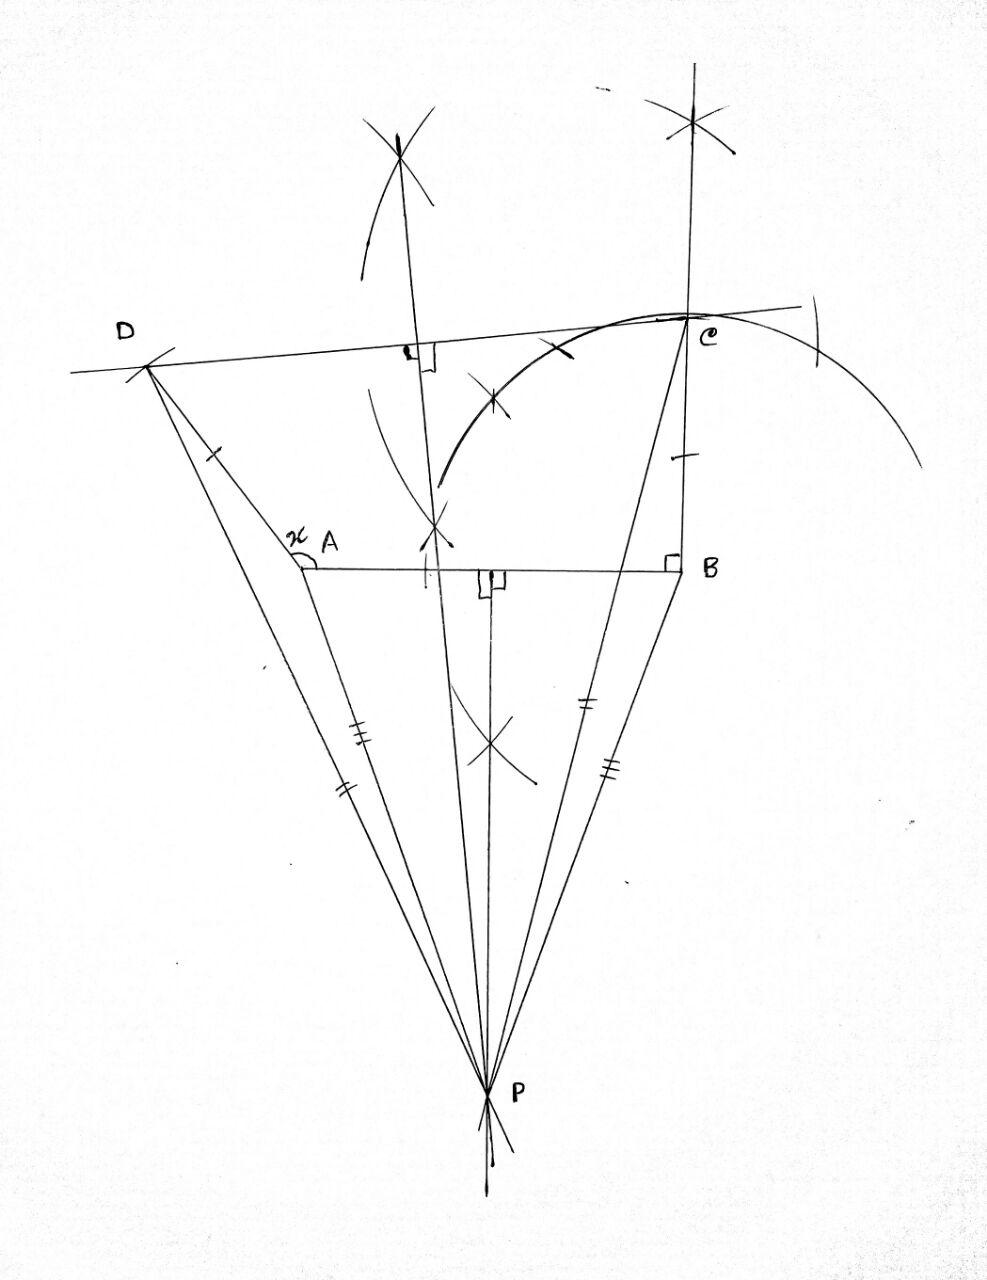
\includegraphics[width=12cm, height=15cm]{images/a.jpg}
\end{figure}

Because unlike the figure in the question, $PD$ will be  outside the quadrilateral $ABCD$. So $\angle PAD-\angle PAB$ does not equals to $x$.
\pagebreak

\item Here it will be easy to solve the problem by Euler's  Totient Function

I learned about Euler's  Totient Function from \footnote{\url{https://en.wikipedia.org/wiki/Euler\%27s_totient_function }}  and from\footnote{An Excursion In Mathematics by M. R. Modak, S. A. Katre, V. V. Acharya and V. M. Sholapurkar}

Another approach is to apply Inclusion–Exclusion Principle but that approach is easy for less number of primes.

I learned about this principle from \footnote{\url{https://en.wikipedia.org/wiki/Inclusion\%E2\%80\%93exclusion_principle}} and from \footnote{Problem-Solving Strategies by Aurther Engel}

For larger number of primes Euler's  Totient Function is most suitable. Here we can not use directly the fuction so first we need to prove it's properties

Let $\phi (n)$ denotes a function such that $\phi (n)=$ number of positive numbers less than $n$ that  are coprime to $n$ where $n\in \mathbb{N}$

Hence for a prime number $p$, \ $\phi (p)=p-1$

For $p^n$ there are $p^{n-1}$ numbers which divide $p^n$. These numbers are $p, \ p^2, \ p^3, \ \cdots , \ p^{n-1}$

Hence:- $$\phi (p^n)=p^n-p^{n-1}=p^n\left (1-\frac{1}{p} \right )$$

Now, for  two primes $p\ \text{\&} \ q$\ , $\phi (p)=p-1$ and $\phi (q)=q-1$

Hence the number of numbers coprime to $pq$ and less than $pq$ is $(p-1)(q-1) $

Therefore:- $\displaystyle{\phi (pq)=(p-1)(q-1)=\phi (p)\phi (q)}$

Let $n$ be a positive number and $n=p_1^{a_1}p_2^{a_2}\cdots p_k^{a_k}$ be the prime distribution of $n$.

Hence:- $\phi (n)=\phi (p_1^{a_1})\phi (p_2^{a_2})\cdots  \phi (p_k^{a_k})=p_1^{a_1}\left (1-\frac{1}{p_1} \right )p_2^{a_2}\left (1-\frac{1}{p_2} \right )\cdots p_k^{a_k}\left (1-\frac{1}{p_k} \right )$

$$\phi (n)=n\left (1-\frac{1}{p_1} \right )\left (1-\frac{1}{p_2} \right )\cdots \left (1-\frac{1}{p_k} \right )$$

The L.C.M. of 2, 3, 5 is $=30$

Hence the number of quite prime positive integers less than 30 is $=\phi (30)=(2-1)(3-1)(5-1)=8$

\underline{First Part} :-

Hence $=\phi (90)=3\times \phi (30)=24$

Now between 90 and 100 there exist 3 quite prime positive numbers

Hence the number of quite prime positive integers less than 100 is $24+4=27$ [Ans]
\bigskip

\bigskip


Now, the number of quite prime positive integers less than 960 is

\ \ \ \ \ \ \ \ \ \ \ \ \ \ \ \ \ \ \ \ \ \ \ \ \ \ \ \ \ \ \ \ \ \ \ \ \  \ \ \ \ \ \ \ \ \ \ \ \ \ \ \ \ \ \ \ \ \ \ \ \ \ \  \ \ \ \ \ \ \ $=\phi (960)=32\times \phi (30)=256$

Now between 960 and 1000 eliminating all the even numbers :-

\begin{center}
  \begin{tabular}{c c c c c}
961 & 963 & 965 & 967 & 969 \\ 
971 & 973 & 975 & 977 & 979 \\ 
981 & 983 & 985 & 987 & 989 \\ 
991 & 993 & 995 & 997 & 999 
   \end{tabular}
\end{center}

Now simply striking out the multiples of 3 then 5 :-
\begin{center}
  \begin{tabular}{c c c c c}
961 & \cancel{963} & \cancel{965} & 967 & \cancel{969} \\ 
971 & 973 & \cancel{975} & 977 & 979 \\ 
\cancel{981} & 983 & \cancel{985} & \cancel{987} & 989 \\ 
991 & \cancel{993} & \cancel{995} & 997 & \cancel{999}
  \end{tabular}
\end{center}

Hence the number of very quite prime positive integers less than 1000 $=256+10=266$ [Ans]
\bigskip

\bigskip

\bigskip

\bigskip

\bigskip

\underline{Second Part} :-

The primes less than 15 are 2, 3, 5, 7, 11, 13

Their L.C.M. $=2\times 3\times 5\times 7\times 11\times 13=30030$

Hence the number of very quite prime positive integers less than $ 30030$ is

\ \ \ \ \ \ \ \ \ \ \ \ \ \ \ \ \ \ \ \ \ \ \ \ \ \ \ \ \ \ \ \ \ \ \ \ \ \ \ \ \ \ \ \ \ \ \ \ \ \ \ \ \ \ $=\phi (30030)=(2-1)(3-1)(5-1)(7-1)(11-1)(13-1)=5760$

Therefore $\phi (90090)=3\times \phi (30030)=3\times 5760=17280$

We need to consider less than 90000

Now from 90001 to 90090 eliminating all the even number we get:-

\begin{center}
  \begin{tabular}{c c c c c c c c c}
90001& 90011& 90021 &90031 &90041& 90051& 90061& 90071 &90081 \\ 
90003& 90013 &90023 &90033 &90043& 90053 &90063 &90073 &90083 \\ 
90005 &90015& 90025& 90035& 90045& 90055 &90065& 90075& 90085 \\ 
90007& 90017& 90027& 90037 &90047 &90057& 90067 &90077 &90087 \\ 
90009& 90019& 90029& 90039 &90049 &90059 &90069 &90079& 90089 
   \end{tabular}
\end{center}
Now simply striking out the multiples of 3 then 5 then 7 then 11 and then 13 :-
\begin{center}
  \begin{tabular}{c c c c c c c c c}
90001 & 90011 & \cancel{90021} & 90031 & \cancel{90041} & \cancel{90051} & 90061 & 90071 & \cancel{90081} \\ 
\cancel{90003} & \cancel{90013} & 90023 & \cancel{90033} & 90043 & 90053 & \cancel{90063} & 90073 & \cancel{90083} \\ 
\cancel{90005} & \cancel{90015} & \cancel{90025} & \cancel{90035} & \cancel{90045} & \cancel{90055} & \cancel{90065} & \cancel{90075} & \cancel{90085} \\ 
90007 & 90017 & \cancel{90027} & 90037 & 90047 & \cancel{90057} & 90067 & \cancel{90077} & \cancel{90087} \\ 
\cancel{90009} & 90019 & 90029 & \cancel{90039} & 90049 & 90059 & \cancel{90069} & \cancel{90079} & 90089 
  \end{tabular}
\end{center}
Hence between 90000  and 90090 there exists 19 very quite prime positive integers present 

Hence  there are $17280-19=17261$ very quite prime positive integers present less than 90000
\bigskip

\bigskip

In general we can say the number of very quite prime positive integers less than a number $n$ is approximately $=\displaystyle{\frac{\phi (30030)}{30030}\times n}$ 
\bigskip

\bigskip


Hence  the number of very quite prime positive integers less than $10^{10}$ is $\approx \displaystyle{\frac{\phi (30030)}{30030}\times 10^{10}} $ [Ans]

\bigskip

\bigskip


And the number of very quite prime positive integers less than $10^{100}$ is  $\approx \displaystyle{\frac{\phi (30030)}{30030}\times 10^{100}} $ [Ans]


\pagebreak

\item Here the monkey have to fill in the $n\times n$ grid in such a way that the cat and the dog have same set of numbers that is the set of 3 numbers obtained by multiplying the numbers in each row is equals to the set of 3 numbers obtained by multiplying the numbers in each column.

A solution for the $3\times 3$ grid ;-
\begin{center}
  \begin{tabular}{| c | c | c |}
     \hline
     9 & 2 & 4 \\
     \hline
     1 & 5 & 6 \\
     \hline
     8 & 3 & 7 \\
     \hline
  \end{tabular}
\end{center}

Hence for $3\times 3$ grid it is possible to arrange the numbers

For $5\times 5$ grid a solution is :-

\begin{center}
  \begin{tabular}{| c | c | c | c | c |}
     \hline
     17 & 2 & 7 & 15 & 20 \\
     \hline
     14 & 25 & 9 & 11 & 16 \\
     \hline
     6 & 21 & 13 & 3 & 12 \\
     \hline
    10 & 22 & 18 & 23 & 1 \\
     \hline
     5 & 24 & 4 & 8 & 19  \\
     \hline
  \end{tabular}
\end{center}

Hence $5\times 5$ has a solution

From the arrangements we can conclude the primes $p$ which have only one multiple which is its own value that is $\displaystyle{\frac{n^2}{2}<p<n^2}$ would be placed at the diagonal [Here only one of the two diagonals can be used]

If the number of such primes is greater than $n$ then it has no solution.

For $11\times 11$ grid the number of primes between 60 to 121 is greater than 11. Hence $11\times 11$ grid has no solution

For $n\times n$ grid the condition on $n$ is $$\left |\{p\ : \ p \ \text{is a prime such that}\ \frac{n^2}{2}<p<n^2 \}\right |<n $$

 Now we can progress further using the Prime Number Theorem\footnote{\url{https://en.wikipedia.org/wiki/Prime_number_theorem}}

Let $\pi (x)$ denotes the prime computing fuction.

That means :- $$\pi (x)= \text{The number of primes less than or equal to}\  x\ \text{where}\ x\in \mathbb{R}$$

Now, with the help of the third inequality under the section of Non-asymptotic bounds on the prime-counting function in \footnote{ \url{https://en.wikipedia.org/wiki/Prime_number_theorem\#Non-asymptotic_bounds_on_the_prime-counting_function}} which states that :-

\ \ \ \ \ \ \ \ \ \ \ \ \ \ \ \ \ \ \ \ \ \ \ \ \ \ \ \ \ \ \ \ \ \ \ \ $\displaystyle{\frac{x}{\log x +2}<\pi (x)<\frac{x}{\log x -4} \ \forall \ x\geq 55 \ \text{where}\ x\in \mathbb{R}} \cdots (1)$

we can find any bound for $n$.

Now,
$$
\frac{n^2}{\log(n^2)+2} - \frac{\frac{n^2}{2}}{\log\left(\frac{n^2}{2}\right) - 4}  > n $$

This inequality is satisfied by $n=11,\ 12, \ 13, \ \cdots 18$.

Now consider the function :-
$$f(x)=\frac{x^2}{\log(x^2)+2} - \frac{\frac{x^2}{2}}{\log\left(\frac{x^2}{2}\right) - 4}-x$$

The graph of the function :-

\begin{figure}[h]
  \centering
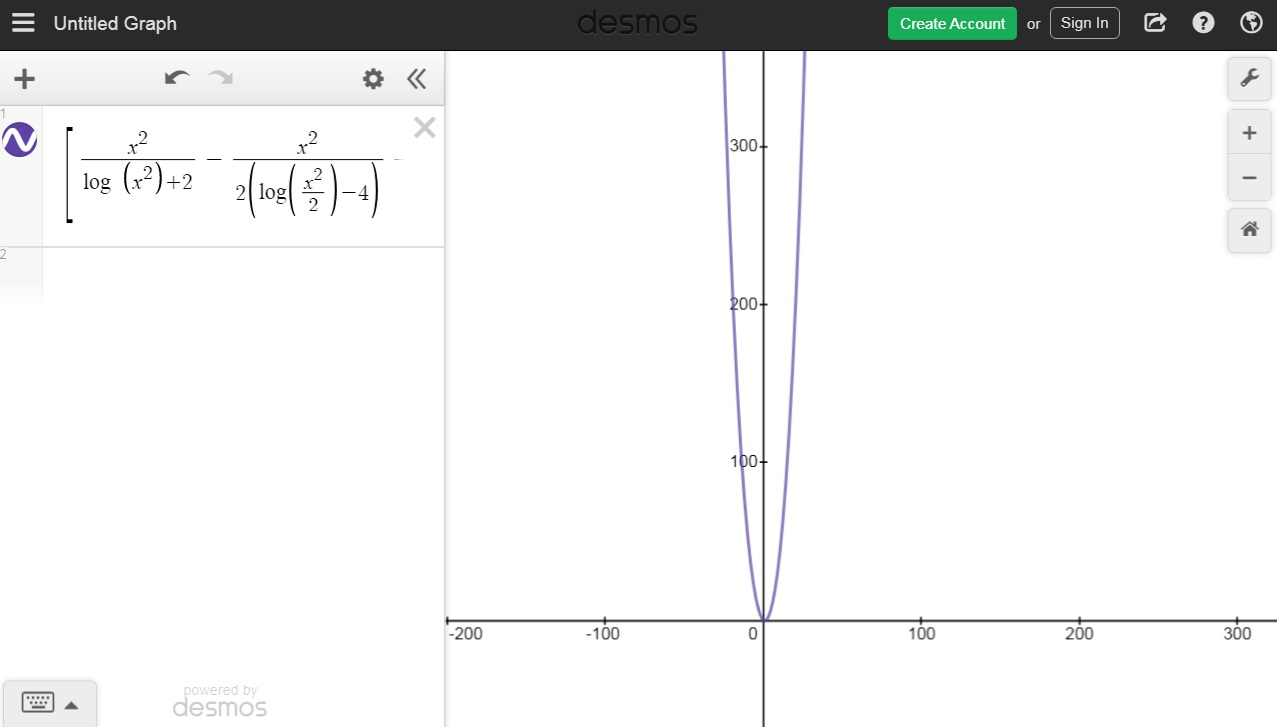
\includegraphics[width=15cm, height=8cm]{images/c.jpg}
\end{figure}

Now, I am unable to prove that this function is always greater than 0 when $x\geq 11$

If it is proven then we can conclude that there is no solution for an $n\times n$ grid  so that the cat and the dog obtain the same set of numbers.

\bigskip

\bigskip

\bigskip

\bigskip

\bigskip



\item The set $S$ contains some real numbers following the 3 rules

  \begin{enumerate}
      \item $1\in S$
      \item If $\frac{a}{b}\in S$ [where $\frac{a}{b}$ is in lowest forms and $a,b $ are coprime] then  $\frac{a}{2b} \in S$
      \item $\frac{a}{b}, \ \frac{c}{d} \in S$ [where $\frac{a}{b}$ and $ \frac{c}{d}$ is in lowest forms and $a,b $  and $c,d $ are coprimes] then $\frac{a+c}{b+d}\in S$
   \end{enumerate}
   
As $1\in S$ hence $\frac{1}{2},\ \frac{1}{4},\ \frac{1}{8}\cdots \in S$
   
Hence till now S contains 1 and some fractions $\frac{a}{b}$ where $a< b$

Now we need to prove that by  those rules a rational number $\frac{p}{q}$ where $p>q$ does not belongs to S
   
Let a fraction  $\frac{m}{n}$ which is less than 1  is in $S$

Hence $\frac{m+1}{n+1}$ also is in $S$ 

$$\frac{m}{n}<1 \implies m<n \implies m+1<n+1\implies \frac{m+1}{n+1}<1$$

Hence with the 3rd rule there can not be a fraction greater than 1 belongs to $S$.

Now in second rule a fraction is halfed and the new fraction is in $S$. 
   
Let a fraction  $\frac{x}{y}$ which is less  than 1  is in $S$   

$$\frac{x}{y}<1\implies x<y\implies x<2y\implies \frac{x}{2y}<1$$

Hence  it is proved that $S$ does not contains any rational number greater than 1.

Hence $S=\{ x \ : x\in (0, \ 1)\ \text{where}\ x\in \mathbb{Q}\}$
\bigskip

\bigskip

\bigskip

\bigskip

\bigskip


\item Let the side of the triangle is $a$.

Now, the area of the triangle is $10$

Hence $\displaystyle{\frac {\sqrt3}{4}}a^2=10$

\ \ \ \ \ \ \ or, $a^2=\displaystyle{\frac{40}{\sqrt3}}$

\begin{figure}[h]
  \centering
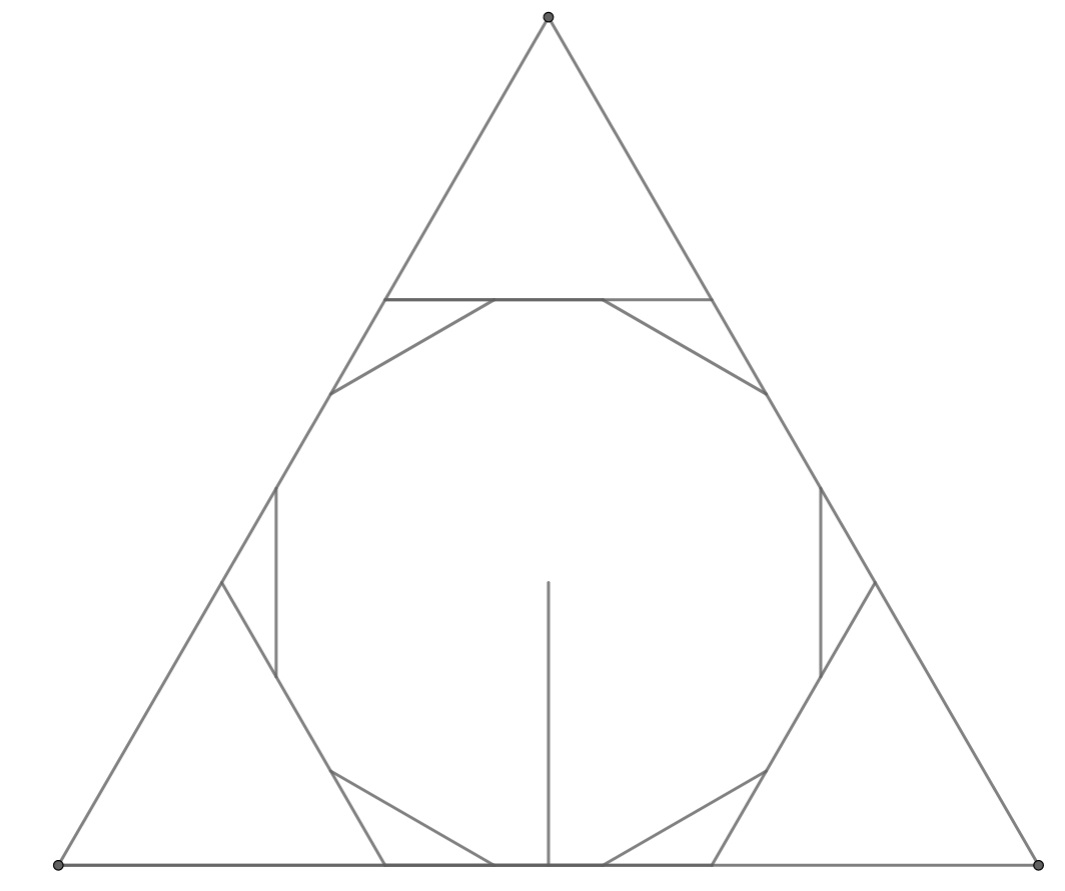
\includegraphics[width=6cm, height=5cm]{images/b.jpg}
\end{figure}

Now after every trisection of sides of previous figure and snipping out the corners a regular polygon is created and the distance between the centre of the polygon and the sides remain same.

Hence $P_1$ is a regular hexagon with side $\displaystyle{\frac{a}{3}}$

The distance between the centre and the sides $= \displaystyle{\frac{\sqrt 3}{2}a\times \frac{1}{3}=\frac{a}{2\sqrt3}}$

Hence area of $P_1$:-
$$P_1=6\displaystyle{\times \frac{1}{2}\times  \frac{a}{2\sqrt3} \times 2\frac{a}{2\sqrt3}  \tan \left(\frac{2 \pi}{2\times 6} \right)}= \frac{a^2}{2}\tan \frac{\pi}{6}=\frac{40}{\sqrt3}\times \frac{1}{2}\times \frac{1}{\sqrt3}=\frac{20}{3}$$

Now, $P_2$ is a regular polygon with 12 sides formed as mentioned above.

Area of $P_2$:-
$$P_2 = 12\times \frac{a^2}{12}\tan \left(\frac{2 \pi}{2\times 12} \right)=\frac{40}{\sqrt{3}}\tan \frac{\pi}{12} $$

After every trisection of the sides of the previous polygon and snipping out the corner the number of sides of the new polygon is twice the previous one.

Hence $P_n $ has $3\times 2^{n-1}$ sides.

In this way the figure tends to reduce into the incircle of the given equilateral triangle.

Hence area of $P_{\infty}$ or $P_n$ where $n \to \infty$ :-
$$ P_{\infty}= \lim \limits_{n \to \infty} P_n = \lim \limits_{n \to \infty} 3\times 2^{n-1}\times \frac{a^2}{12}\tan \left(\frac{2 \pi }{2\times 3\times 2^{n-1}} \right)=\lim \limits_{n \to \infty} 3\times 2^{n-1}\times \frac{a^2}{12} \tan \left(\frac{ \pi}{ 3\times 2^{n-1}}\right)$$

$$=  \lim \limits_{n \to \infty}\frac{a^2}{12}\times \frac{\tan \left(\frac{ \pi}{ 3\times 2^{n-1}}\right)}{\frac{\pi }{3\times 2^{n-1}}}\times \pi = \pi \times \frac{a^2}{12}=\pi \times \frac{40}{\sqrt{3}}\times \frac{1}{12}= \frac{10\pi}{3\sqrt{3}} $$

$P_{\infty}$ or $P_n$ where $n \to \infty$ is the incircle of the equilateral triangle.

Hence the area of $P_{\infty}=$ Area of the incircle $=\displaystyle{\frac{10\pi}{3\sqrt{3}}}$. 
\bigskip

\bigskip

\bigskip

\bigskip

\bigskip

\setcounter{enumi}{9}
\item For 3 trains :-
\begin{center}
  \begin{tabular}{c | c}
    Final remaining linked up trains & Number of times from all possible arrangements \\
    \hline
    1 & 2 \\
    2 & 3 \\
    3 & 1 \\
  \end{tabular}
 \end{center} 
Hence average of all outcomes $=\displaystyle{\frac{1\times 2+ 2\times 3+ 3\times 1}{3!}=\frac{11}{6}=1+\frac{1}{2}+\frac{1}{3}}$

For 4 trains :-
\begin{center}
    

  \begin{tabular}{c | c}
    Final remaining linked up trains & Number of times from all possible arrangements \\
    \hline
    1 & 6 \\
    2 & 11 \\
    3 & 6 \\
    4 & 1
  \end{tabular}
\end{center}
Hence average of all outcomes$=\displaystyle{\frac{1\times 6+ 2\times 11+ 3\times 6+4\times 1}{4!}=\frac{50}{24}=1+\frac{1}{2}+\frac{1}{3}+\frac{1}{4}}$

Noticing the pattern in case of 5 trains average of all outcomes may be $=\displaystyle{1+\frac{1}{2}+\frac{1}{3}+\frac{1}{4}+\frac{1}{5}}$
\bigskip

\bigskip

Let $C(n)$ be avarage of all outcomes when there are $n$ trains in the line. 

We need to prove that $$C(n)=\sum \limits_{i=1}^n \frac{1}{i}$$

Let this is true for $n=k$

Hence $$C(k)=\sum \limits_{i=1}^k \frac{1}{i}$$

For $n=k+1$ we can say that a new train is introduced behind all the k trains in case of $n=k$

Let $v_1,\ v_2,\cdots,\ v_k$ denotes the speeds of the $k$ trains where $v_1>v_2>\cdots >V_k$

Hence there are $(n+1)$ intervals of speeds; $(\infty,\ v_1]$,  $(v_1,\ v_2]$,  $(v_2,\ v_3]$, $\cdots$,  $(v_k,\ 0)$ 

Therefore the speed of $(k+1)$th train can be from any of these intervals 

The slowest train and the trains behind it forms a cluster which is always at the tail end. Then  the trains between the slowest and the second slowest  trains forms a cluster with the second slowest train and so on

Now two cases arise :-
  \begin{enumerate}
      \item The speed of $(k+1)$th train is less than $v_k$. Then  the $(k+1)$th train will form a single cluster of its own. 
      
      The probability of this event $=\displaystyle{\frac{1}{n+1}}$ as the speed of $(k+1)$th train only belongs to $(v_k,\ 0)$
      \item The speed of $(k+1)$th train is more than slowest train. Then it will join the last cluster.
      
      The probability for this event is $=\displaystyle{\frac{n}{n+1}}$ as the speed of $(k+1)$th train belongs to any of the intervals $(v_1,\ v_2]$, $(v_2,\ v_3],\ \cdots$, $(v_{k-1},\ v_k]$
      \end{enumerate}
      
Hence $$C(k+1)= \frac{C(k)+1}{n+1}+\frac{C(k)\times n}{n+1}=C(k)\left(\frac{1}{n+1}+\frac{n}{n+1} \right)+\frac{1}{n+1}=C(k)+\frac{1}{n+1}$$

Hence by Mathematical Induction we can say that $C(n)=\displaystyle{\sum \limits_{i=1}^n \frac{1}{i}}$ is true for all $n\geq3$ [Proved]

Therefore $C(5)=\displaystyle{1+\frac{1}{2}+\frac{1}{3}+\frac{1}{4}+\frac{1}{5}}$
  
Hence for $n$ trains average of all possible outcomes  $=\displaystyle{\sum \limits_{i=1}^n \frac{1}{i}}$


\begin{flushright}
\vspace*{\fill}
Typed in \LaTeX
\end{flushright}






\end{enumerate}
\end{document} 